\section{多质点体系的引力作用}\label{sec:04.07}

我们知道,牛顿的万有引力定律式\eqref{eqn:04.03.04}
\begin{equation}\label{eqn:04.07.01}
	F = \frac { G m _ { 1 } m _ { 2 } } { r ^ { 2 } }
\end{equation}
是对两个质点而言的。牛顿在发展引力理论过程中,重要的一步
是把月亮运动和落体运动统一起来。在这个分析中,一个关键的
问题是牛顿认为地球表面落体运动的加速度可以写为
\begin{equation}\label{eqn:04.07.02}
	g = \frac { G M _ \text{地} } { R ^ { 2 } }
\end{equation}
其中$ R $是地球半径。其实式\eqref{eqn:04.07.02}是直接从式\eqref{eqn:04.07.01}得来的。
这里有一个很大的疑问,为什么能把地球和落体间的距离看为$ R $?
如果说在讨论月亮运动时,把地球和月亮看作质点是一个足够好
的近似,那么讨论落体运动时,把地球看作质点显然是不合理的
\begin{wrapfigure}[11]{r}{17em}
	\centering
	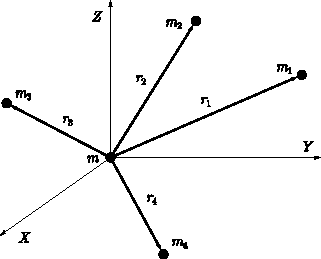
\includegraphics{figure/fig04.09}
	\caption{多质点体系的引力}
	\label{fig:04.09}
\end{wrapfigure}
牛顿一开始就意识到这一点,他感到不加证明地取地球和落体间距离
为R,从理论上来说是有欠缺的。后来,他给出了严格的证明。为了
研究这个问题,我们必须来讨论一下多质点体系的引力问题。

现在我们先来讨论一种简单情况。如图\ref{fig:04.09}~
% 145.jpg
所示,在原点有一质量为m的质点,空间分布着质量分别为$ m _ { 1 } $,
$ m _ { 2 } $,$ m _ { 3 } $,$ \cdots $,$ m _ { i } $的若干个质点,它们的位置矢径分别为$ r _ { 1 } $,$ r _ { 2 } $,$
r _ { 3 } $,$ \cdots $, $ r _ { i } $。为了求质点$ m $所受到的引力,必须把式\eqref{eqn:04.07.01}作
些推广。根据式\eqref{eqn:04.07.01}可知:
{\setlength{\mathindent}{2em}
\begin{equation}\label{eqn:04.07.03}
	\begin{aligned}
\mbox{}&\text{第一个质点对}\,m\,\text{的引力为}
 & \vec{F} _ { 1 } = \frac { G m m _ { 1 } } { r _ 1 ^ { 2 } } \cdot \frac { \vec{r} _ { 1 } } { r _ { 1 } } \\
\mbox{}&\text{第二个质点对}\,m\,\text{的引力为}
& \vec{F} _ { 2 } = \frac { G m m _ { 2 } } { r _ 2 ^ { 2 } } \cdot \frac { \vec{r} _ { 2 } } { r _ { 2 } } \\
\mbox{}&\cdots \cdots \cdots \cdots \\
\mbox{}&\text{第}\;i\;\text{个质点对}\,m\,\text{的引力为}
& \vec{F} _ { i } = \frac { G m m _ { i } } { r _ i ^ { 2 } } \cdot \frac { \vec{r} _ { i } } { r _ { i } } \\
\end{aligned}
\end{equation}}
式中$ \frac { \vec{r} _ { i } } { r _ { i } } $表示第$ i $个质点对$ m $的引力的方向。因此,可以自然地认
为,$ m $所受到的总力为
\begin{equation}\label{eqn:04.07.04}
	\begin{aligned}
\erratanote{\ensuremath{\vec{F}}}{\ensuremath{\vec{F}_1}} &=  \vec{F} _ { 1 } + \vec{F} _ { 2 } + \cdots + \vec{F} _ { i } \\
&= \sum _ i { \frac { G m m _ { i } } { r _ { i } ^ 2 } \cdot \frac { \vec{r} _ { i } } { r _ { i } } }
\end{aligned}
\end{equation}

应当指出,这个推广中暗含了一个新观点。式\eqref{eqn:04.07.04}并不
全同于\eqref{eqn:04.07.01}所包含的物理内容,因为式\eqref{eqn:04.07.01}只说了两个质
点间的引力作用,而式\eqref{eqn:04.07.04}的写法,在本质上是认为两质点之
间的引力作用只与这两质点有关,而与第三者、第四者等等是否
存在毫无关系,可以不加顾及。这个新的物理内容是引力的一个
重要性质,我们称之为引力的线性迭加性。并不是所有的力都有
这种性质,譬如,强相互作用就没有这种性质。

做了上述推广,就可以来讨论牛顿所遇到的问题了。

考虑一密度均匀的球壳(图\ref{fig:04.10}),它的厚度$ t $比它的半径$  $r
小得多。我们要求出它对球壳外一个质量为$ m $的质点$ P $的引力。

可以把球壳看成许多小块的集合,每个小块在$ P $点上都有作
% 146.jpg
用力,这力的大小应当与该小块的质量成正比,而与它和$ P $点之
间的距离的平方成反比,方向沿着它们之间的连线。然后,我们
再求球壳上所有部分对$ P $点的合力。
\begin{figurex}
 \centering
 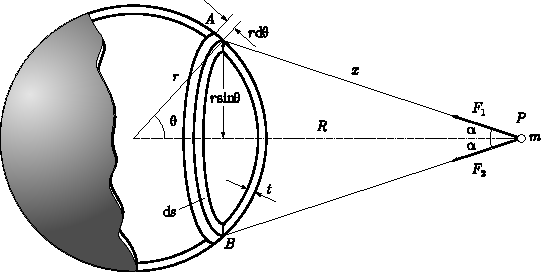
\includegraphics{figure/fig04.10}
 \caption{球壳的引力}
 \label{fig:04.10}
\end{figurex}\vspace{-0.5em}

%{\renewcommand{\CJKglue}{\hskip 0pt plus 0.09pt}
设在球壳\,$ A $\,点处的一小块对\,$ m $\,的引力为\,$ \vec{F} _ { 1 } $,由球壳的对称性,
我们可以找到与\,$ A $\,相对称的\,$ B $\,点,该处的一小块对\,$ m $\,的引力为\,$ \vec{F} _ { 2 } $\,。
由于对称,故\,$ \vec{F} _ { 1 } $\,与\,$ \vec{F} _ { 2 } $\,这两个力的竖直分量彼此抵消,而水平分量
\,$ F _ { 1 } \cos \alpha $\,与\,$ F _ { 2 } \cos \alpha $\,相等。通过把球壳分为这样一对一对的小块,我
们立刻可以看出,所有作用在\,$ m $\,上的力的竖直分量都成对地相互
抵消了。为了求出球壳对\,$ m $\,的合引力,我们只需考虑水平分量。
%}

如图\ref{fig:04.10},考虑球壳上的一环带,该环带长为$ 2 \uppi ( r \sin \theta ) $,宽
为$ r d \theta $,厚为$ t $。因此,它的体积为
\begin{equation*}
 \dif V = 2 \uppi t r ^ { 2 } \sin \theta \dif \theta
\end{equation*}
设密度为$ \rho $,则环带的质量为
\begin{equation*}
 \dif M = \rho \dif V = 2 \uppi t \rho r ^ { 2 } \sin \theta \dif \theta
\end{equation*}
$ \dif M $对位于$ P $点处的质量$ m $所施的力是水平的,其值为
%\begin{equation}\label{eqn:04.07.05}
% \begin{aligned}
% \dif F &= G \frac { m \dif M } { x ^ { 2 } } \cos \alpha \\
% & = 2 \uppi G t \rho m r ^ { 2 } \frac { \sin \theta \dif \theta } { x ^ { 2 } } \cos \alpha
% \end{aligned}
%\end{equation}
\begin{equation*}
        \dif F = G \frac { m \dif M } { x ^ { 2 } } \cos \alpha \\
\end{equation*}
\begin{equation}\label{eqn:04.07.05}
        \mbox{} \qquad = 2 \uppi G t \rho m r ^ { 2 } \frac { \sin \theta \dif \theta } { x ^ { 2 } } \cos \alpha
\end{equation}
% 147.jpg
其中$ x $,$ \alpha $和$ \theta $之间满足下列关系
\begin{equation}\label{eqn:04.07.06}
 \cos \alpha = \frac { ( R - r \cos \theta ) } { x }
\end{equation}
再根据余弦定理
\begin{equation}\label{eqn:04.07.07}
 x ^ { 2 } = R ^ { 2 } + r ^ { 2 } - 2 R r \cos \theta
\end{equation}
即
\begin{equation}\label{eqn:04.07.08}
 r \cos \theta = \frac { R ^ { 2 } + r ^ { 2 } - x ^ { 2 } } { 2 R }
\end{equation}
对式\eqref{eqn:04.07.06}进行微分,得
\begin{equation*}
 2 x \dif x = 2 R r \sin \theta \dif \theta
\end{equation*}
即
\begin{equation}\label{eqn:04.07.09}
 \sin \theta \dif \theta = \frac { x } { R r } \dif x
\end{equation}
将式\eqref{eqn:04.07.08}代入式\eqref{eqn:04.07.06},再将式\eqref{eqn:04.07.06}、\eqref{eqn:04.07.09}代入式
\eqref{eqn:04.07.05},从而消去$ \theta $与$ \alpha $,得
\begin{equation}\label{eqn:04.07.10}
 \dif F = \left( \frac { \uppi G t \rho m r } { R ^ { 2 } } \right) \left( \frac { R ^ { 2 } - r ^ { 2 } } { x ^ { 2 } } + 1 \right) \dif x
\end{equation}
这就是环带$ \dif S $的物质作用在质点$ m $上的引力。

整个球壳的作用即为上式对所有环带求和,亦即对变量$ x $求
遍及整个球壳的积分。因为$ x $的范围是从最小值$ R - r $到最大值
$ R + r $,所以
\begin{equation}\label{eqn:04.07.11}
 \int _ { R - r } ^ { R + r } \left( \frac { R ^ { 2 } - r ^ { 2 } } { x ^ { 2 } } + 1 \right) \dif x = 4 r
\end{equation}
故合力为
\begin{equation*}
 \begin{aligned}
 F &= \int _ { R - r } ^ { R + r } \dif F \\
&= G \frac { ( 4 \uppi r ^ { 2 } \rho t ) m } { R ^ { 2 } } \\
% 148.jpg
 \end{aligned}
\end{equation*}
\begin{equation}\label{eqn:04.07.12}
    \mbox \quad = G \frac { M m } { R ^ { 2 } }
\end{equation}
式中$ M = 4 \uppi r ^ { 2 } t \rho $为球壳的总质量。这个结果表明,一个密度均匀
的球壳对球壳外一质点的引力,等效于它的所有质量都集中于它
的中心时的引力。

一个实心球体可当作由大量同心球壳所构成。如果各层球壳
具有不同密度,但每一球壳都具有均匀密度,则同样的论证也适
用于这种实心球体。因此,对于象地球、月球或太阳这类近似于
球体的天体来说,在讨论它们的吸引力时,就可以把它们当作质
量集中在球心的质点来处理。

应当强调,之所以有上述结果,是我们用了引力的迭加性和
引力的距离平方反比律。因此上述结果对其他类型的力就不一定
成立。

其实,地球并不是标准的球体,而是有点象梨的形状,“梨”
的较小一端在北半球。因此,式\eqref{eqn:04.07.12}是不严格的。若考虑地
球的真实形状,引力表达式将非常复杂。譬如,在地球附近运行
\begin{wrapfigure}[11]{r}{16em}
    \vspace{-0.5em}
 \centering
 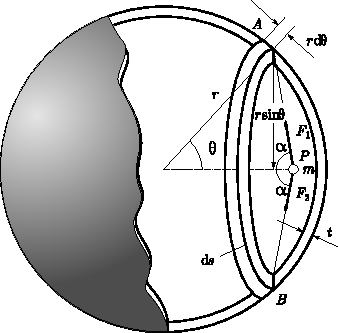
\includegraphics{figure/fig04.11}
 \caption{对球壳内部的引力}
 \label{fig:04.11}
\end{wrapfigure}
的人造地球卫星,明显地偏离了开普勒定律所
描述的轨道。实际上,现代的研究正是利用了
这一点。我们是反过来,由人造地球卫星实
际轨道对开普勒定律的偏离,来研究地球的形
状和质量的分布。

另一个有意义的结果是,球壳对内部任一
质点的引力为零。以下
% 149.jpg
我们参照图\ref{fig:04.11}来证明这个论断。

现在,$ m $位于球壳内部,即$ R $小于$ r $,因而式\eqref{eqn:04.07.10}以及式
\eqref{eqn:04.07.11}仍然适用,但其积分限应换成从$  r - R   $到$  r + R  $,即
\begin{equation*}
    \int _ { r - R } ^ { r + R } \left( \frac { R ^ { 2 } - r ^ { 2 } } { x ^ { 2 } } + 1 \right) \dif x = 0
\end{equation*}
所以\vspace{-1.56em}
\begin{equation*}
    F = 0
\end{equation*}
这个结果有很大的意义,我们将在下章讨论。